In this section, the layer is described in some detail in terms of its specific subsystems. Describe each of the layers and its subsystems in a separate chapter/major subsection of this document. The content of each subsystem description should be similar. Include in this section any special considerations and/or trade-offs considered for the approach you have chosen.

\subsection{Application Sub-System}
The application subsystem is the Graphical User Interface that interacts with the user to get user inputs if necessary and sends it to the database in form of a query.

\begin{figure}[h!]
	\centering
 	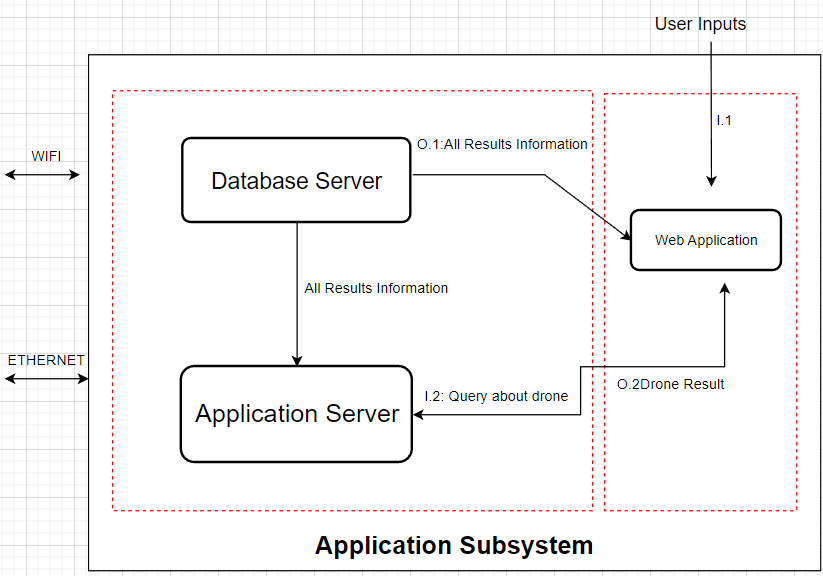
\includegraphics[width=0.70\textwidth]{images/Application_Subsystem.png}
 \caption{Data flow of Application Subsystem}
\end{figure}

\subsubsection{Assumptions}
For the operation of this subsystem, it is assumed that the user has access to WIFI or some form of internet and a browser to launch the web application.

\subsubsection{Responsibilities}
This subsystem is responsible for the database interaction with the user. First of all, the data of all the detected drone is displayed to the user then if the user requests for more information on a particular drone then the request is forwarded to the database in form of a query and the database results are displayed. 

\subsubsection{Subsystem Interfaces}

\begin {table}[H]
\caption {Subsystem interfaces} 
\begin{center}
    \begin{tabular}{ | p{1cm} | p{6cm} | p{3cm} | p{3cm} |}
    \hline
    ID & Description & Inputs & Outputs \\ \hline
    \#I.1 & User Inputs & \pbox{3cm}{Click on particular drone title} & \pbox{3cm}{Query to the database about the drone}  \\ \hline
     \#I.2 & Query about drone & \pbox{3cm}{The query to the database} & \pbox{3cm}{Results according to the query}  \\ \hline
    \#O.1 & List of objects & \pbox{3cm}{N/A} & \pbox{3cm}{List of drone and non drone objects}  \\ \hline
    \end{tabular}
\end{center}
\end{table}

\subsection{Subsystem 2}
Repeat for each subsystem

\subsection{Subsystem 3}
Repeat for each subsystem

